\documentclass{beamer}
\setbeamercovered{transparent}
\usepackage{epstopdf}
\usepackage{listings}
\usepackage{lipsum}
\usepackage{subfig}
\usepackage{algorithm}
\usepackage{algorithmicx}
\usepackage{cite}
\usepackage{lipsum}
\usepackage{amssymb}
\usepackage{color}
\usepackage{IEEEtrantools}
\usepackage{booktabs}
\usepackage{texpower}
\usepackage{amsmath}
\usepackage{caption}
\usepackage{multirow}
\usepackage{graphicx}
\newtheorem{Key points}{Key points}
\newtheorem{Summary}{Summary}
\usepackage{dblfloatfix}
%\usepackage{adjustbox}
%\usepackage{animate}
%\usepackage{movie15}
%\usepackage{subfig}
%\newtheorem{Definition}{Definition}
%\usepackage[font={small}]{caption}
\usepackage{beamerthemeshadow}
\newcommand\Fontvi{\fontsize{5}{6.2}\selectfont}
\newcommand\Fontvia{\fontsize{6}{7.2}\selectfont}
\newcommand\Fontviaa{\fontsize{8}{7.2}\selectfont}
\usepackage{listings}
\lstset{language=C++,
                keywordstyle=\color{blue},
                stringstyle=\color{red},
                commentstyle=\color{green},
                morecomment=[l][\color{magenta}]{\#},
                numbers=left,
                escapeinside=||
}

%\captionsetup{font=scriptsize,labelfont=scriptsize}
 \usetheme{Antibes}%PaloAlto
\begin{document}
\title[Lecture 1]{Data Structures} 
\author[]{Ahsan Ijaz}
\date{}
 \frame{\titlepage}
% \AtBeginSection[]
% {
% \begin{frame}<beamer>{Table of Contents}
% \tableofcontents[currentsection,currentsubsection, 
%     hideothersubsections, 
%     sectionstyle=show/shaded,
% ]
% \end{frame}
% }
\section{Data Structures}
\frame{\frametitle{Data Structures}
A data structure is designed to organize data to suit a specific purpose so that it can be accessed and worked with in appropriate ways. 

  \begin{itemize}
\item \textbf{Fixed-size} data structures have fixed size assigned to them at compile time
one-dimensional arrays,two-dimensional arrays and structs. 
\item \textbf{Dynamic data structures}  grow and shrink during execution.
  \end{itemize}
}
\subsection{Dynamic Data Structures}
\frame{\frametitle{Dynamic Data Structures}
  \begin{itemize}
  \item Linked Lists
  \item Stacks
  \item Queues
  \item Trees
  \end{itemize}
}

\frame{\frametitle{Stacks}
  \begin{itemize}
  \item Stacks are important in compilers and operating systems:
    Insertions and removals are made only at one end of a stack, its
    top.
  \end{itemize}
  \begin{figure}
    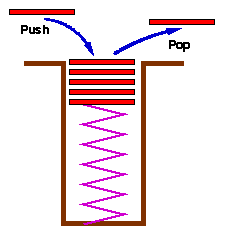
\includegraphics[width=0.25\columnwidth]{stack}
  \end{figure}
} \frame{\frametitle{Linked Lists}
  \begin{itemize}
  \item Linked lists are collections of data items lined up in a
    row. Insertions and removals can be made anywhere in a linked
    list.
  \end{itemize}
  \vspace{\fill}
  \begin{figure}
    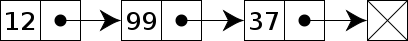
\includegraphics[width=0.5\columnwidth]{linked}
  \end{figure}
  \vspace{\fill} }

\frame{\frametitle{Queues}
  \begin{itemize}
  \item Queues represent waiting lines; insertions are made at the
    back (also referred to as the tail) of a queue and removals are
    made from the front (also referred to as the head) of a
    queue. This makes the queue \emph{a First-In-First-Out (FIFO)}
    data structure.
  \end{itemize}
  \vspace{\fill}
  \begin{figure}
    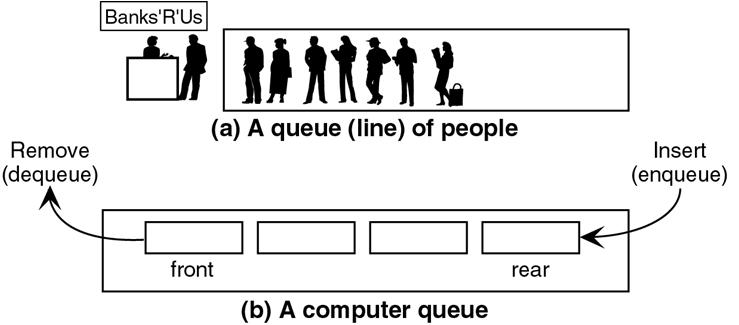
\includegraphics[width=0.7\columnwidth]{queues}
  \end{figure}
  \vspace{\fill} }

\frame{\frametitle{Trees}
  \begin{itemize}
  \item Trees facilitate high-speed searching and sorting of data and
    efficient elimination of duplicate data items. It imitates a
    hierarchical tree structure set of linked nodes which are ordered
    and directed and each node has zero or more children.
  \end{itemize}
  \vspace{\fill}
  \begin{figure}
    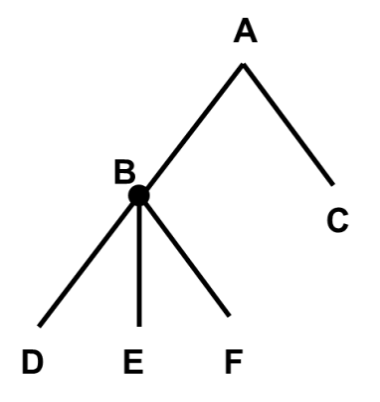
\includegraphics[width=0.3\columnwidth]{tree}
  \end{figure}
  \vspace{\fill} }

\frame{\frametitle{Graph}
  \begin{itemize}
  \item A graph data structure consists of a finite set of ordered pairs, called edges, of certain entities called nodes or vertices. 
  \end{itemize}
  \vspace{\fill}
  \begin{figure}
    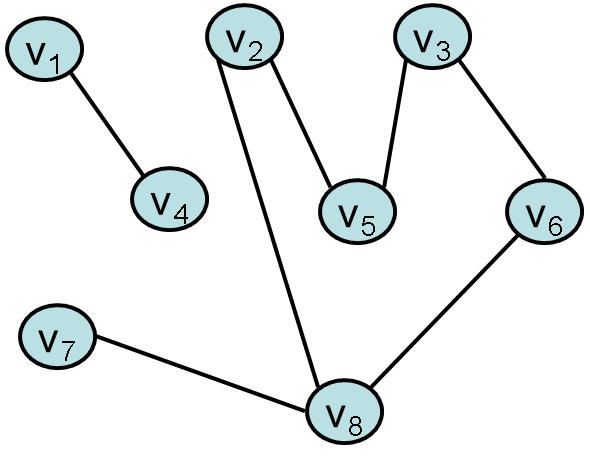
\includegraphics[width=0.7\columnwidth]{graph}
  \end{figure}
  \vspace{\fill} }

\section{Self referential Classes}
\frame{\frametitle{Self Referential Classes}
  \begin{itemize}
  \item A self-referential class contains a pointer member that points to a class object of the same class type. 
  \end{itemize}
}
\begin{frame}[fragile]
\frametitle{Class Declaration}
\Fontviaa
\begin{lstlisting}
class Node
{
public:

    Node( int ); // constructor
    void setData( int ); // set data member
    int getData() const; // get data member
    void setNextPtr( Node * ); // set pointer to next Node
    Node *getNextPtr() const; // get pointer to next Node

 private:

    int data; // data stored in this Node
    Node *nextPtr; // pointer to another object of same type

}; // end class Node
\end{lstlisting}
\end{frame}

\frame{\frametitle{Self Referential Classes}
  \begin{itemize}
  \item A class Node has two private data members; \textbf{integer member data} and \textbf{pointer member nextPtr}.\\
\item Member nextPtr points to an object of type \textbf{{\color{red}Node}}.
  \begin{itemize}
  \item It is another object of the same type as the one being declared here, hence the term "self-referential class”.
  \end{itemize}
\item Member {\color{red}\textbf{nextPtr}} is referred to as a \textbf{link}.\\
  \begin{itemize}
  \item i.e. \textbf{nextPtr} can "tie" an object of type Node to another object of the same type. 
  \end{itemize}
  \end{itemize}

}

\frame{\frametitle{Self Referential Classes}
  \begin{itemize}
  \item For a linked data structure, the last node in the link must be set to null.
\item Self-referential class objects can be linked together to form useful data structures such as lists, queues, stacks and trees.
  \end{itemize}
}

\frame{\frametitle{Self Referential Classes}
  \begin{figure}
    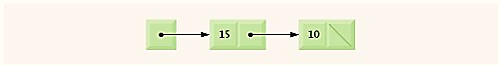
\includegraphics[width=0.9\columnwidth]{selfcl}
\caption{two self-referential class objects linked together to form a list. }
  \end{figure}
 \begin{itemize}
  \item The slash represents a null (0) pointer placed in the link member of the second self-referential class object to indicate that the link does not point to another object. 
\item A null pointer indicates the end of a data structure.
  \end{itemize}

}
\frame{\frametitle{Dynamic Memory Allocation and Data Structures}
 \begin{itemize}
  \item Creating and maintaining dynamic data structures requires \emph{dynamic memory allocation}.
\item When that memory is no longer needed by the program, it can be released so that it can be reused to allocate other objects in the future. 
  \end{itemize}

}


\end{document}